\section{Introduction}
\label{industry_needs}
As we mentioned in chapter \ref{chapter_general_intro}, despite the main aim of this thesis has been to derive a methodology for approximating the motivational state of individuals while interacting with a potentially rewarding object (a videogame in this case), a secondary objective was to illustrate the potential application of this methodology within an industrial setting. 

In this view, this chapter will focus on sketching the design of a system relying on our methodology for automated engagement prediction and quantification. First, we will provide an overview on why a company might need a process for quantifying and predicting engagement and which characteristics this process should have. Then, we will proceed at illustrating a system designed for serving this need, placing particular emphasis on how its components connect with the work presented so far. Finally, we will introduce a set of ethical considerations that should be taken into account when designing such system.

\section{Automated Engagement Quantification and Prediction}
\label{industry_needs}
In an industry setting the development of research projects often aims at the the resolution of specific problems or at the improvement processes central to success (be it measure in terms of revenues or perceived quality of goods and services). 

So where does engagement quantification and prediction sits within the needs of the videogame industry? Very often (if not always) the success of a videogame title is strictly connected with either its ability to retain users or with the experience that users had with the product (i.e., a videogame title) \cite{amit2001value, alomari2016mobile}. The first is pivotal in scenarios where games are treated as a service sold to an audience (similarly to the function of streaming services) while the second is more relevant in situations where games are to be considered digital goods \cite{amit2001value, alomari2016mobile}. 

In this context, engagement can be viewed as a measure of how a particular game was, is or will be able to retain users. For example, if an individual is engaged with a particular service (e.g., a videogame) it is likely that will keep paying a subscription (or any other form of pay-to-consume) for said service. Similarly, if an individual had a good experience with a particular digital good, it is more likely that they will promote it to other potential users, acquire similar products or buy products from the same seller.  

In this view being able to predict the propensity that a user (or a group of users) has towards a particular game translates (in a more or less direct way) to the capacity of assessing if a game is likely to be a success of public and revenue. For this reason it is often the case that videogame publishers and studios try to leverage the information they have available through telemetry systems for taking the stock of how a particular game is performing \cite{el2016game}. 

This is a classical example of analytical reports summarizing various type of Key Performance Indicators (KPI)\cite{el2016game} or profiling techniques describing how users interacted with a particular game \cite{el2016game}. Despite this approaches are very relevant for gathering insights on the performance of a particular game title, they only allow to execute what we call "reactive" interventions. By reactive interventions we mean that mitigating actions for improving a sub-optimal situation (e.g., when a videogame is unable to foster engagement) can only be taken \textit{ex-post}.

On the other hand, interventions based on the outcomes of a predictive model are by definition "pro-active". This is because knowing in advance if a particular situation is going to be problematic or not allows one to plan and deliver mitigating actions \textit{ex-ante} \cite{el2016game, el2021game}. It is worth noticing that approaches based on the outcome of predictive models are not incompatible with techniques used within a "reactive" framework (e.g., reports and profiles) but rather complementary. For example, the same KPI calculated on observed data can and should be computed also on predictions and forecasts generated by a machine-learned model. Similarly, it is possible to create profiles that not just describe the historical interactions of users with a particular game but that are also informative of the expected future engagement of such users. Within this last "pro-active" framework lies the work that we presented in this thesis. 

\section{System prototype Design}
\label{pipeline}

In this section we will proceed at illustrating the design of a system prototype aimed at delivering predictions and insights that can foster \textit{ex-ante} interventions for the mitigation and improvement of videogames engagement. 

We will pose particular attention on the fact that our proposed system is designed to rely on a "global model" \cite{wang2019deep} suitable for application in multi-contexts scenarios. Examples of such scenarios includes situations in which a single large entity (e.g., a publisher) manages multiple videogame titles or when multiple small players (e.g., independent studios) decide to form a consortium. We will also illustrate how our system encompasses not only the three tasks mentioned so far, namely: prediction, reporting and profiling, but also allow to generate representations that can be used as inputs to other machine-learning systems. 

A diagram illustrating the proposed design for our system prototype is presented in Figure \ref{pipeline}:

\begin{figure}[ht]
\centering
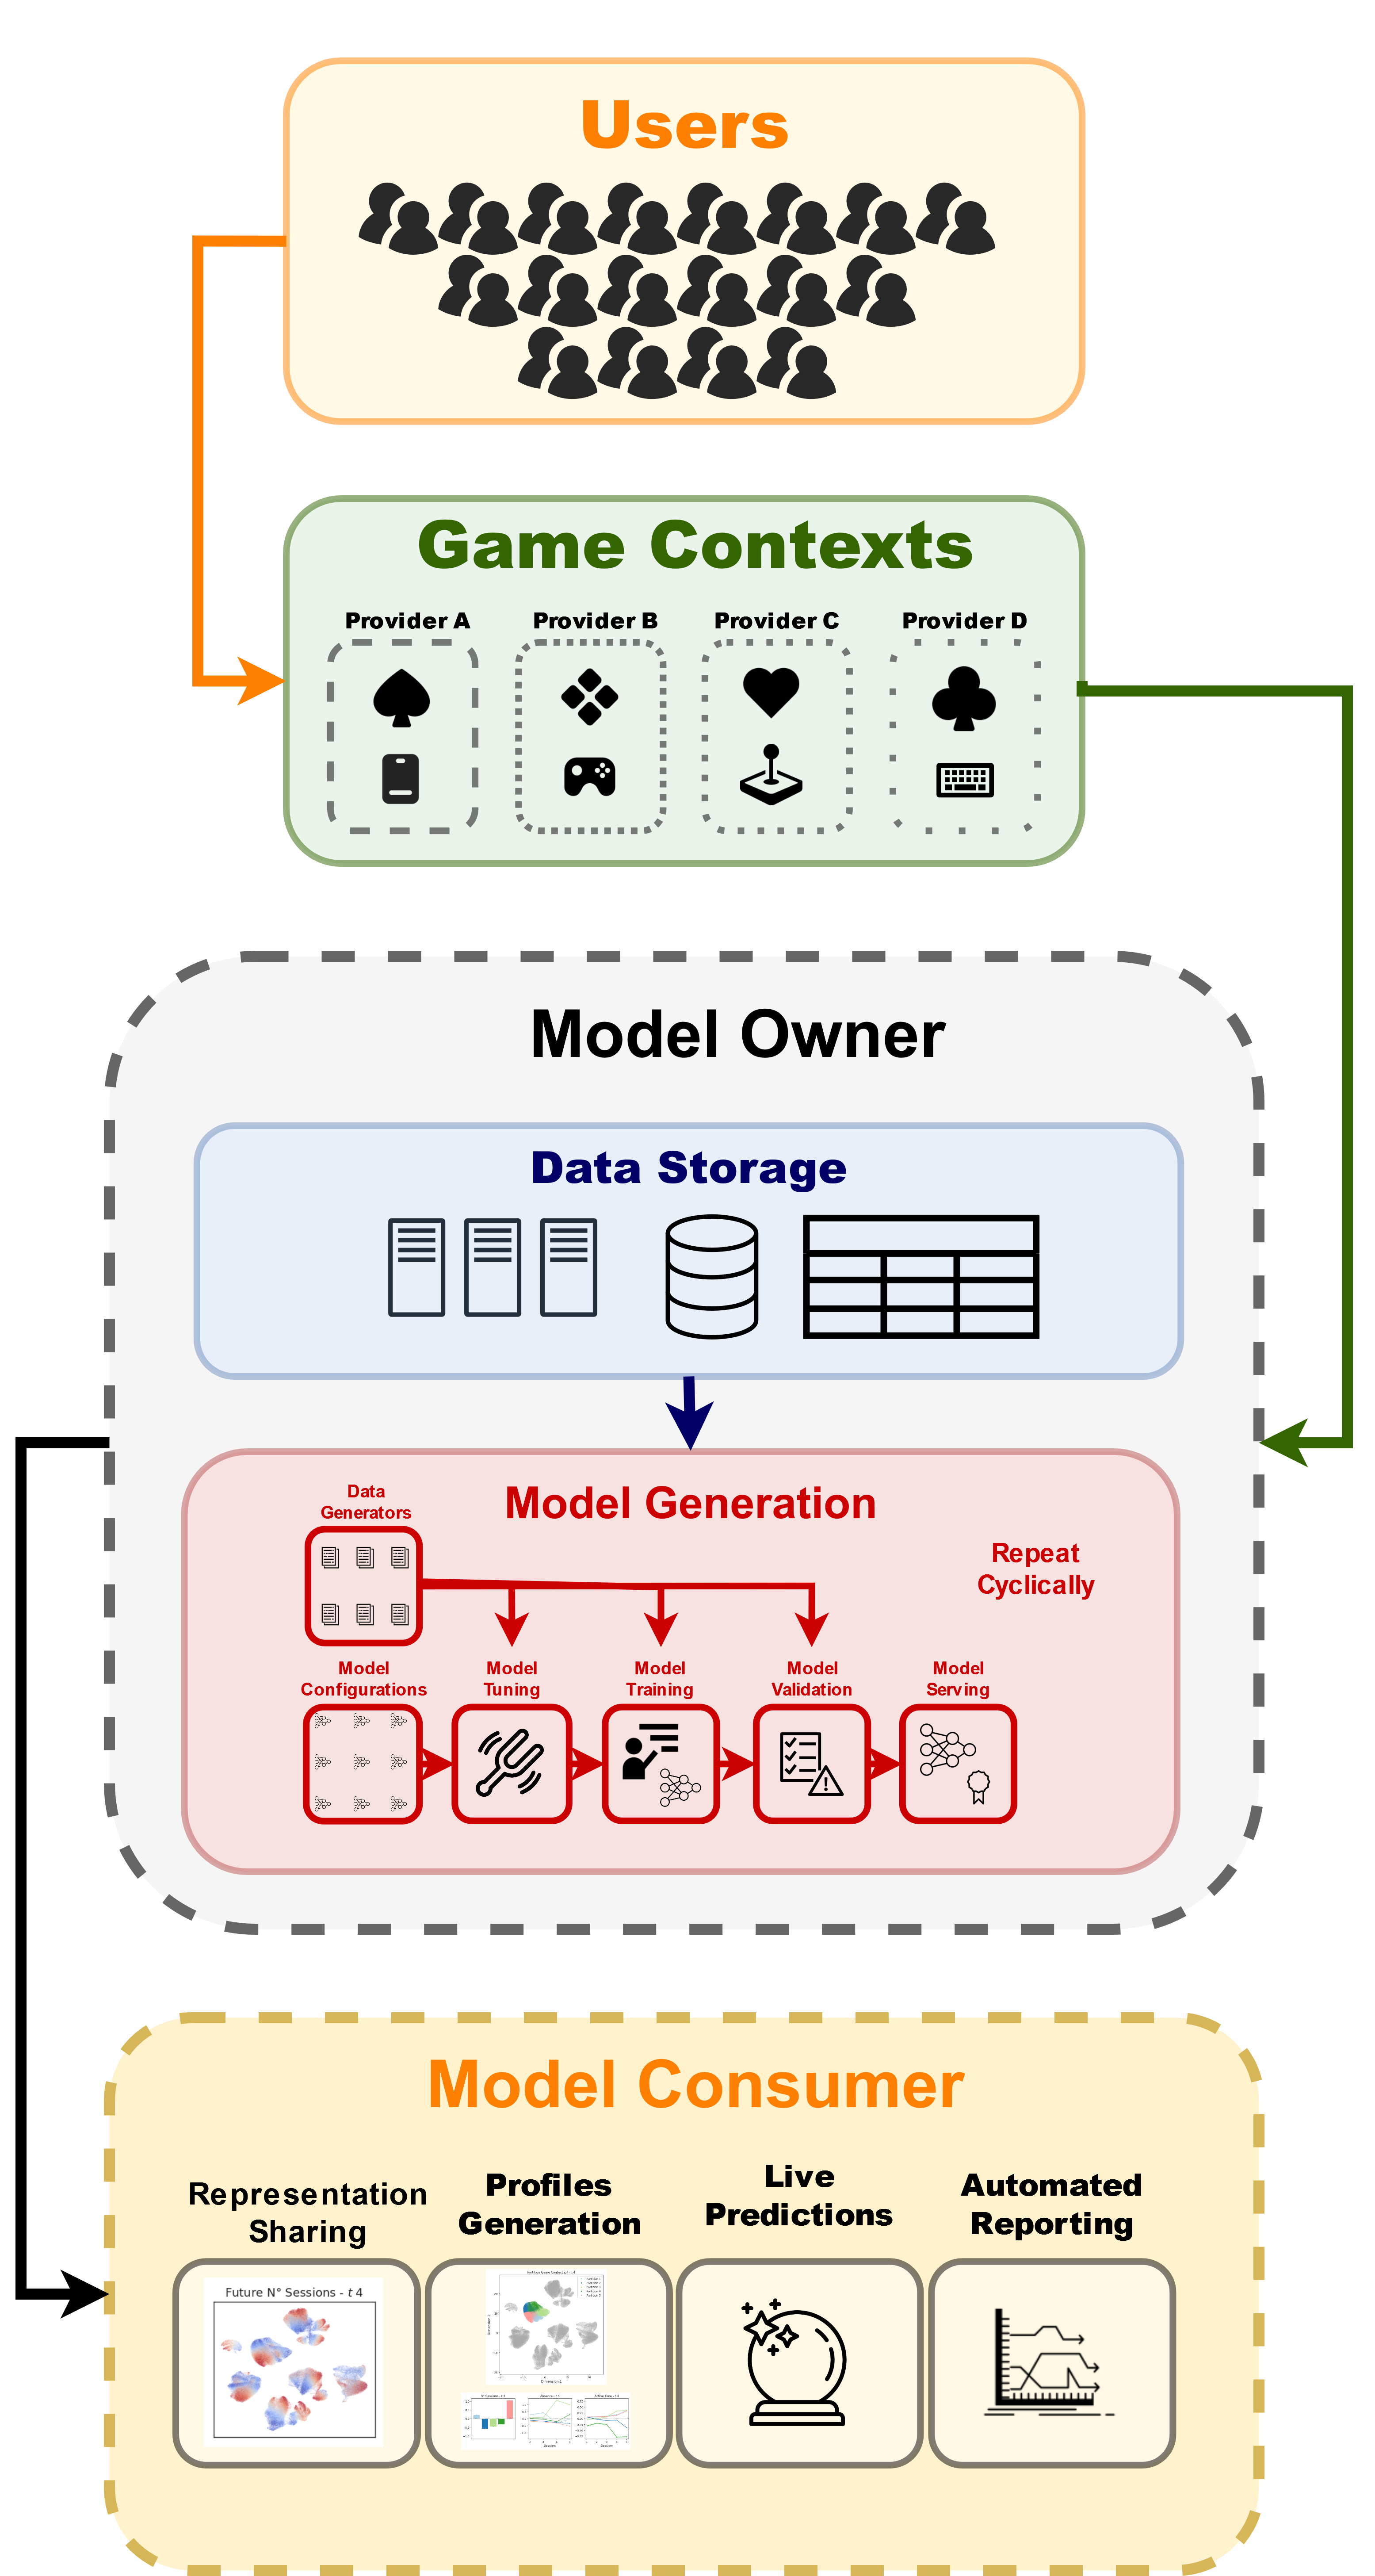
\includegraphics[width=0.5\textwidth]{images/chapter_5/pipeline_diagram.png}
\caption[\textbf{Engagement Prediction and Quantification - System prototype Design Diagram}]{The figure represents a simplified system diagram for a potential application of the improved RNN architecture presented in section \ref{model_architecture_3}. Solid lines indicate low-level components in the system while dashed lines indicate high-level entities. Directional arrows represent the flow of operations inside the system.}
\label{pipeline}
\end{figure}

It is worth noticing that we will focus on illustrating the various components presented in Figure \ref{pipeline} but we will not describe the type of interventions that can be taken on the basis of the system's outputs. Indeed this, other than being an articulated and complex subject that in itself would require an additional research project, is outside the scope of the current work. The responsibility and knowledge required for designing, executing and evaluating interventions ultimately sits within those entities consuming the output the model.

\subsection{Data Generation}
\label{data_generation}
This is the first component of the system and describes the entities generating the data that will then be used by the system. It is composed by two major elements: the users and the game contexts. By users we mean the pool of individuals that already had an interaction with one or more of the considered game contexts. With game contexts we extend the definition of game object presented in \ref{chapter_theory_modelling} in order to include not just the game world but also the elements necessary for making the interface with the users possible (i.e., software and the hardware components). In the interest of simplicity and for better connecting this section to the work described in chapters \ref{chapter_lit_review} and \ref{chapter_theory_modelling}, we invite to consider user and game context as aliases for individuals and game objects.

In line with the framework that we adopted through out this thesis we assume that each game context possesses properties (defined by their structural characteristics) that might result to be more or less rewarding to different users. By means of repeated interactions with the game contexts the users learn about these properties and progressively updates latent representations of the various contexts. These representations, which as we said in chapters \ref{chapter_lit_review} and \ref{chapter_theory_modelling} are imbued with value, act by either promoting or demoting future engagement with the game contexts (net of the contribution of the surrounding environment). The amount of engagement can be measured, form a behavioural point of view, by means of metrics indicative of the frequency and intensity of the playing behaviour.

The various game contexts can be managed by a single or multiple entities (e.g., publishers, studios or public organisations) and can be provided through different type of hardware. For example, the game contexts utilized for this thesis were managed by a single publisher (i.e., our partner company Square Enix Ltd.) and provided through an array of different hardware systems (e.g., smartphones, tablets, personal computers and gaming consoles). Ultimately, the software and console hardware not only generate the game object with which the users interact but also support the telemetry system in charge of recording, processing and transmitting metrics (behavioural and not) to the relevant data storage systems.

\subsection{Model Owner}
\label{model_owner}
This component of the system represents the entity responsible for the acquisition and storage of telemetry data generated by the interactions between the users and the game contexts. It is also in charge of managing all the operations necessary for fitting a learning algorithm to the data and validating the derived model. 

It is relevant to highlight that the model owner usually corresponds one-to-one with the entity managing the game contexts (or components of the game contexts) but the two do not necessarily have to coincide. In the context of federated learning  \cite{yang2019federated} for instance, a model owner might distribute copies of the same learning algorithm across separate entities and only act as a pooling mechanism  once they have been fitted to the data \cite{kairouz2021advances}. In this case, the entities do not necessarily need to be known to the model owner or to each other, in fact this information must be kept hidden. In this view, federated learning allows to generate robust global models (like the architecture presented in this thesis) by fitting a learning algorithm on heterogeneous data distributed across a large number of independent actors \cite{yang2019federated, kairouz2021advances}. Moreover, since the aim of federated learning is to generate such models while being compliant with strict privacy constrains \cite{yang2019federated, kairouz2021advances}, this opens to the possibility of collaborations between competitors (e.g., consortium of small private companies) or neutral entities subjected to strict data sharing limitations (e.g., research institutions).

That said, for simplicity in this section we will focus on a situation where the model owner coincides with the entity managing the game contexts.

\subsubsection{Data Storage}
\label{data_storage}
Once the in-game behaviour resulting from the interaction between the users and the game contexts have been recorded by the telemetry system the information need to be transferred to a suitable storage system. Depending on the needs and technical capacity of the storage owner this can happen either via data streams or batch processing \cite{el2016game}. The component in charge of storing the data should also take care of conducting suitable Extract, Transform and Load (ETL) operations in order to move from the raw format in which the telemetries are collected to a more suitable one employable by the learning algorithm \cite{el2016game}. The ETL operations should also take care of all those data validation, sanity checks and pre-processing steps that are not directly relevant to the generation of the machine-learned model. This would correspond to the various filters and data munging operations that we mentioned in sections \ref{data_1}, \ref{data_2} and \ref{data_3}.

\subsubsection{Model Generation}
\label{model_generation}
Once the raw information provided by the telemetry system has been processed, cleaned, organised and stored in a suitable format a learning algorithm can be fitted to the data. In this case we assume the learning algorithm to be one of the three ANN architectures presented in chapter \ref{chapter_implementation_testing} and hence relying on the same operations presented in sections \ref{tuning_comparison_1}, \ref{tuning_comparison_2} and \ref{tuning_comparison_3} for tuning, fitting and validating.

\paragraph*{Data Generators} the first step in the model generation require the construction of appropriate mechanisms for feeding the data to the learning algorithm. Different generators will need to be created for the various steps of the process: one for tuning, one for training (i.e., fitting) and one for validating the generated model. It is worth noticing that the data generators do not only need to provide batches of the data to learning algorithm but are also in charge of: 

\begin{itemize}
    \item Applying the appropriated transformations (e.g., input scaling) in such a way that no information leaking is occurring.
    \item Individuate and satisfy relevant stratification needs required for having a representative sample of the target population.
    \item Adopt adequate randomisation and splitting strategies to avoid introducing biases during the model fitting.
\end{itemize}

\paragraph*{Model Configurations} simultaneous to the construction of the data generators is the creation of multiple architectural configurations for the learning algorithm. This step assume the use of a tuning algorithm similar to HyperBand \cite{li2017hyperband} for the search of the optimal hyperparameters. Indeed, as we specified in chapter \ref{chapter_implementation_testing} HyperBand works by iteratively training a large pool of models instantiated with a random selection of hyperparameters and progressively pruning those showing poor out-of-sample perfromance. At this stage the only thing that needs to be specified are the hyperparameters to optimize and the boundaries of the search space. Routinely validation checks should also be included in this stage for removing from the pool of potential configurations those that resulted to be corrupted. Indeed certain hyperparameters configurations might make training or even model instantiation infeasible.

\paragraph*{Model Tuning} once the model configurations have been generated it is possible to search for the best performing hyperparameters. Despite in this work we leveraged the HyperBand algorithm \cite{li2017hyperband}, other type of tuning algorithm can be taken into consideration.  The choice of which tuning algorithm to chose should be informed by the problems at hand along with eventual time and resources constrains. For example, methods based on surrogate models like Gaussian Processes \cite{bergstra2011algorithms} are effective but expensive and complex approaches. On the other hand methods relying on naive random search despite their lack of efficiency are cheap and straightforward to implement. It is worth noticing that at this stage not just the hyperparameters relative to the architecture can be optimized but also those associated with other components used during the training stage (e.g., the optimizer learning rate). The amount of data assigned to the data generator used at this stage should strike a balance between efficacy and waste. If too little data are used, the hyperparameters search might produce sub-optimal results. However, going to the other extreme might hurt the training stage as the data used for searching the best model configuration cannot be re-used. Another piece of information that needs to be specified is the amount of computational budget to be given to the tuning algorithm a choice that again be informed by the available resources and time constrains.

\paragraph*{Model Training} at this stage the best model configuration should be fitted to the bulk of the available data. It is worth noticing that depending on the size of the training data this stage might be very resource intensive. However, model fitting should not necessarily always be carried out on the entire amount of data. For example, if the algorithm has recently been through a full training stage (e.g., leveraging all the available historical data) an update based on the latest available data might be sufficient. Moreover, if significant resource constraints are present, it might be possible to fit the learning algorithm using a suitably defined random sample of the original data. This of course depends on the number of parameters in the model, the complexity of the learning task and the heterogeneity and size of the available data. Fitting the model to the data should be carried out until convergence or a suitably defined level of accuracy is achieved, again the choice of such level might be dictated by time or resource constraints. In this regard, convergence should always be assessed and monitored through out-of-sample metrics with the option of triggering an early stopping policy if improvements are not observed for a long period of time (see details specified in sections \ref{tuning_comparison_1}, \ref{tuning_comparison_2}, \ref{tuning_comparison_3}). What is important at this stage is to create checkpoints of the model state whenever out-of-sample accuracy reliably improves and to keep detailed logs of the fitting procedure. The first avoids wasting efforts if the optimisation process suddenly diverges or come to an abrupt end (e.g., due to technical issues), the second allows keeping track of relevant metrics useful for assessing if and how convergence is reached.

\paragraph*{Model Validation} once the learning algorithm has been fitted on the data it is necessary to validate it in order to verify its usability in a production environment. The validation process can be extremely articulated and in large part depends on the needs of the model owner, however, two main aspects should certainly be validated. First, a series of tests should be conducted in order to verify that basic functionalities are not disrupted, in our case for example we might want to make sure that the model is able to produce predictions and representations, that these are within critical boundaries (e.g., no extremely large or small values are present) and show particular properties (e.g., statistical or distributional ones). Second, the convergence and accuracy of the model should be assessed and compared against a critical lower bound or the performance of a naive approach (we provided some examples of these in sections \ref{competing_models_1}, \ref{competing_models_2} and \ref{competing_models_3}). Convergence can be assessed by running automated tests on the logs created during Model Training, checking for example the difference between in-sample and out-of-sample performance, variations in the performance$l2$ norm of the error gradient or in the values of the parameters \footnote{We suggest to consult \cite{bengio2017deep} for a more exhaustive list of checks}. Accuracy can be evaluated by assessing model performance on a test set and then comparing it against the aforementioned benchmarks. In this case, statistical approaches based on inference can be used for evaluating if the expected gains provided by the model lie outside of a Region Of Practical Equivalence (ROPE) and can justify the cost associated to deploy the model in production (an example of this can be found in Appendix \ref{appendix_ancillary_perf}).

\paragraph*{Model Serving} once the model has been validated it is possible to deploy it within a production environment. The frequency at which the model is queried for obtaining predictions or representation depends on the needs of the model consumer and again the available resources. For example, a demanding streaming approach might be needed for supporting live predictions or a system aiming to react to a rapid turnover of large volumes of users. On the other hand, a conventional scheduled job executing a prediction pipeline on a much more relaxed schedule (e.g., once a day or even once a week) might be more than sufficient for generating static KPI reports and updating user profiles. The model generation process should be repeated end-to-end on a regular basis depending on how much distributional drift is expected in the data. However, parts of it like Model Training, Validation and Serving might be executed independently on a much more frequent schedule. 

\subsection{Model Consumer}
\label{model_consumer}
The model consumer identifies the entity interacting with the model and leveraging its outputs. As specified in section \ref{model_owner} this doesn't necessarily have to correspond to the model owner but it is supposed to be identified in at least one of the entities managing the game contexts. Again, for simplicity we will assume that in this case they all corresponds to the same entity. The model consumer shouldn't have direct access to the algorithm generated by the model owner nor should be able to alter its inner working (e.g., it should be able to re-fit the algorithm on a new set of the data), its only focus should be to consume its output for different type of applications. We will now proceed at briefly illustrating some examples of these applications.

\subsubsection{Representation Sharing}
\label{represenation_sharing}
As we described in chapters \ref{chapter_theory_modelling} and \ref{chapter_repr_anal}, the latent representation inferred by the different types of RNN architectures can be thought as an approximation of the saliency that an individual has attributed to the act of interacting with a specific a game context. We can think of it as compressed trace of the state of a user (or a group of users) indicative of the amount of their future engagement. 

As we have seen in section \ref{representation_env_even_contr}, this representation can be constructed from different types of inputs, being them the intensity of historical interactions with the game context or the sequences of game mechanics with which a user interacted. In this view, it can be seen as a set of features extracted by the ANN architectures (see sections \ref{artificial_neural_networks} and \ref{manifold_learning}) which can then be made available to other learning algorithms in order to improve their perfromance. 

For example, a representation generated from game events metric (see section \ref{representation_env_even_contr}) can be interpreted as the set of future answering the question: "which sequences of in-game mechanics are expected to produce higher or lower level of future engagement?". In this view, a recommender system might leverage such representation in order to produced personalized suggestions for contents that are more likely to foster engagement \cite{bertens2018machine}. A prime example of this type of applications is the recent work by Yang et al. \cite{yang2022large}, were the authors proposed a recommender system base on Graph Neural Networks which included a sub-module explicitly designed for engagement modelling. 

Similarly, systems aiming to compute lifetime value (LTV) indexes (which are indicators of the expected profitability of user within a pay-per-play business model) might benefit from a representation informative of the  amount of future gaming behaviour expected by a group of users. Indeed such systems rely on two major components for deriving the LTV index: the avergae expenditure from a group of users along with their expected amount of future engagement \cite{chen2018customer}.

More generally, any automated system indirectly relying on information about the expected level of engagement could benefit from such representation. The reason for this is that by providing "pre-computed" features informative of the level of expected engagement it is possible to alleviate the computational burden of other learning algorithms (or components of a learning algorithm)  which focus should be on solving a potentially different task. This becomes particularly relevant in contexts where the amount and variety of available data make it challenging to perform manual or algorithmic feature selection.

\subsubsection{Profile Generation}
As we have seen in sections \ref{partition_behaviour}, \ref{partition_environment} and \ref{partition_event} it is possible to partition the various representations generated by the ANN architecture in order to obtain corresponding behavioural profiles. These profiles distinguish themselves from those generated in previous work in the literature \cite{drachen2014comparison, bauckhage2012players, makarovych2018like, aung2018predicting} in two fundamental ways:

\begin{enumerate}
    \item They are, by design, able to represent behavioural dynamics (due the recurrent operations used for generating the representation space) within the full history of interactions. It has been common practice in the literature to apply clustering algorithm, sequentially, to time series data \cite{sifa2013behavior,bauckhage2014beyond,aung2018predicting} with no guarantee that the temporal structure was preserved (a notable exception to this is the work by Makarovych et al. \cite{makarovych2018like}).
    \item They are engagement-specific (due to the objective function used for fitting the ANN architecture, more details can be found in section \ref{manifold_learning}) and therefore offer a convenient framework for their interpretation. Other approaches in the literature preferred to adopt completely unsupervised approaches \cite{drachen2014comparison, drachen2012guns} in order to derive more holistic but less specific profiles.
\end{enumerate}

Interrogating the profiles generated from the representation extracted by our approach can provide insights not just on the most frequent sequences of events triggered within a game context, but also on their dynamics and associated level of expected engagement. This can be of use if the model consumer is interested in evaluating how users interacted with the various mechanics as the game progresses \cite{sifa2013behavior, makarovych2018like} and if specific sequences of events are associated with variations in the expected amount of future engagement. 

\subsubsection{Live Predictions}
The most straightforward application of our approach makes use of the predictions generated by the model for solving the conventional tasks of churn and survival time prediction (see chapters \ref{chapter_lit_review} and \ref{chapter_implementation_testing} for a more detailed description of these two tasks). These predictions are conventionally used as the building block for various type of automated decision-making systems such as in-app notifications \cite{milovsevic2017early}, delivery of in-game incentives or targeted marketing campaigns \cite{el2016game, el2021game}. 

The general principle behind these systems is relatively straightforward: the predictions produced by a model are used as an indication of the expected level of future engagement, if this level falls below or above a certain threshold a set of automated mitigating actions are triggered. For example, if a user is predicted to enter in a phase of dis-engagement (see the framework of O'Brien et al. presented in section \ref{eng_proc_model}) a set of small in-game incentives might be issued in the attempt to retain them. On the other hand, if a user is projected to produce a high amount of playing behaviour within a specific game context, a series of messages promoting novel in-game contents could be provided.

In this regard, the methodology presented in this thesis offer a series of technical advantages over previous approaches (see table \ref{eng_model_overview} for an overview of the works on the subject). First, the prediction provided by our model are on a continuous scale allowing the model consumer to chose suitable thresholds for calibrating the triggering of the relevant mitigating actions. Second, instead of providing predictions for a single indicator (e.g., churn probability or survival time) our approach does it so for multiple behavioural metrics (i.e., the five targets presented in section \ref{data_2} and \ref{data_3}) allowing for a more holistic characterisation of the level of expected engagement. Finally, since our model is able to provide credible intervals for its predictions (see section \ref{results_1} for an example of that) it is possible for the model consumer to adopt a more cautious approach, or flat out reject predictions, in situations of high uncertainty.

\subsubsection{Automated Reporting}
As we mentioned in section \ref{industry_needs}, analytical reports covers an important role in the decision making processes taking place within the videogame industry \cite{el2016game}. The inspection of KPI reporting how many users are actively playing a game and how long and frequentl are their interactions can provide a very effective description of how good or bad a game is performing. Moreover, the ability of stratify this indicators according to demographics of interest or ad-hoc business rules makes them extremely versatile tools for individuating potential areas of intervention \cite{el2016game}.

That said, any action taken on the basis of such indicators is bounded to be "reactive" rather than "proactive". In order to circumvent this issue the same type of reports derived from historical data could be generated using the output of a predictive model. For example, it would be possible to monitor the number of users expected to have a marked decrease or increase in future engagement after a major change in the game has been released. Similarly, it would be possible to quantify the number of users projected to have a high or low engagement profile within specific demographic groups, sections of the game or regions of the world. 

What is worth noticing is that all the applications examples illustrated so far can be derived from a single unified framework. This framework  can simulatenously leverage a large amount data sources and serve multiple game contexts. This can in principle alleviate the costs that would be associated to the implementation, maintenance and deployment of multiple systems relying on different learning algorithms (e.g., developing and maintaining a single cross-games pipeline instead generating single ones for each of the available game context). Moreover, fitting a single "global model" on a wide range of game contexts allow to produce representations and predictions that are simultaneously informed by all the available data therefore less prone to "silos effects" (e.g., lack of robustness and generalizability caused by the inability of different models to share information). 

\section{Some Ethical Consideration}
\label{ehtical_considerations}
Automated system leveraging behavioural data are now-days used extensively in both low (e.g., marketing) and high stakes (e.g., credit assessment) scenarios \cite{mehrabi2021survey, dwivedi2021artificial}, with the potential to have a direct and concrete impact on individuals \cite{dwivedi2021artificial}. For this reason, when designing automated data-driven applications, issues related to fairness should be taken into account. 

By fairness we entail the set of principles and considerations that have been adopted recently to avoid that decisions based on a machine-learned model do not inadvertently bring harm to specific groups of people \cite{mehrabi2021survey}. A complete overview of the issue of fairness in machine learning would be beyond the scope of not just this section but the entire thesis, as it is a vast landscape \cite{mehrabi2021survey} hard to navigate due to its many levels of complexity \cite{corbett2018measure}.  We will therefore focus on three major aspects related to the work presented, in this chapter. 

The first aspect concerns biases present in the data on which a machine learning algorithm is fitted. These might be induced by an over or under representation of certain strata of the population that an automated system will ultimately need to serve \cite{mehrabi2021survey}. Given how machine learning algorithms are often fitted to the data (e.g., maximum likelihood) the risk is that their predictions will revert to the mean or in the worst case, will result to be biased with respect to the true characteristics of the population \cite{corbett2018measure, mehrabi2021survey}. Despite the harm that these biases might cause in the context of engagement prediction is not as pronounced as in other areas (e.g., criminal or medical risk assessment), they can still have unexpected repercussion on an individual if they assume that people engage in similar ways regardless of situational, personal and cultural differences. For example an individual might receive notifications in inappropriate contexts (e.g.,  during an emotionally challenging period) or be unfairly penalized within the game world (e.g., due to irregular playing patterns caused by personal or situational reasons) because they deviate from what is the expected behaviour in the data on which the algorithm was fitted.

To this connects the second aspect of fairness that we want to highlight, namely the risk of inadvertently cause harm to individuals which are either temporarily or structurally subject to some form of vulnerability. This might happen as a consequence of automated decision making based on what we call "unconstrained model predictions", what we mean by this is when the predictions from a model are used verbatim without knowing the context in which they will be applied. For example, if we imagine a system aimed at individuating high spending users within a game relying on gacha or loot-box mechanics, relying on unconstrained predictions might in this case inadvertently target individuals with a predisposition to or an history of problematic gambling behaviour \cite{petrovskaya2022prevalence}. The most problematic aspect related to this issue is that often the information required for "constraining" an "unconstrained prediction" are not available to the system, either because they are not easy to derive (e.g., they are not directly observable) or should not be accessible (e.g., they are Personal Identifiable Information - PII \cite{EUdataregulations2018}).

Related to the first two points is the third and final aspect of fairness that we would like to address which is connected with the right to object specified by the General Data Protection and Regulation act (GDPR) \cite{EUdataregulations2018} which allows an individual to object to the processing of their data in any form and at any moment. Despite this aspect it is partially attenuated by rights granted by the GDPR (although this interests exclusively the European Union), it only covers the processing of data rather than the effect connected with automated decision making. An individual might object to the inclusion of their data during the decision making process but still be subject to the effect of this last one, for example, if the system entails a policy of blanket intervention based on the average user behaviour for all those individuals for which no data are available.

As we mentioned at the beginning of the paragraph, an exhaustive treatment of these issues and the relative mitigating actions that could be taken is beyond the scope of the current work. Nevertheless, we want to stress that addressing them in an effective manner is of pivotal importance when automated systems based on machine-learning (or other forms of statistical decision making) becomes part of the operations of a company.

\section{Discussion}
In this chapter we proposed the design of a system aimed at leveraging the modelling approach described chapters \ref{chapter_theory_modelling} and \ref{chapter_implementation_testing} for automated engagement prediction and quantification. We first described why a company (or a consortium of companies) might be interested in such system and why it is important to rely predictive approaches for taking "proactive" actions towards the improvement of user engagement and retention. Subsequently we proceeded at describing the various components of the system trying to connect them with the work presented in the manuscript putting particular attention on providing examples of potential applications. Finally, we highlighted some ethical considerations that should be taken into account when developing and deploying such system. 

It is important to note that this chapter is far from being an exhaustive treatment of the topic, we aimed mostly at illustrating how our approach could be translated in a system designed for satisfying specific needs of the videogame industry. Future work in this area should investigate and expand on a series of topic introduced in this chapter. For example, a more detailed description of the system and its sub-components is needed. This should pose particular attention on the resilience, reliability and efficiency of the system and on the challenges derived by deploying and maintaining it within a suitable production environment. The application examples reported in section \ref{model_consumer} are presented in the form of Proof of Concept (POC) and therefore must be tested within concrete business cases. This is an essential step required for gathering a better understanding of the type and magnitude of impacts that a system like the one we proposed might have. Finally, it would be ideal to illustrate which type of interventions could be carried out on the basis of the outputs of the system. The elaboration, execution and validation of such interventions however can only be the result of a collective endeavour where the designer of the system liaises and leverage the knowledge of various relevant figures within the business: engineers, designers, analysts as well as product and growth managers.


